\phantomsection
%\addcontentsline{toc}{chapter}{Introduzione}
\chapter{Research Study} \label{chapter:research_study}
\markboth{Research Study}{}

\begin{citazione}

\end{citazione}
\newpage

\section{Changes implemented in GreenCloud}\label{section:greencloud_mod}
The modifications made to the \emph{GreenCloud} simulator's code aim to achieve a time-stamped log of the instantaneous overall energy consumption of the Data Center. While exploring the log files, it became apparent that such a report was missing. Therefore, it was necessary to construct it using the data provided by the simulator. As discussed in Subsection \ref{subsection:greencloud_code}, in order to enable scripts to access the variables provided by \emph{C++} classes and create simulation reports, a binding between these variables and symbolic names within the classes is necessary. Since the \emph{SwitchEnergyModel} class defined in the file \href{https://github.com/vincenzo-emanuele/masters-degree-thesis/blob/main/greencloud_modified_src/ns2/greencloud/switchenergymodel.cc}{ns2/greencloud/switchenergymodel.cc} and responsible for modeling switch energy consumption, does not make the \emph{eCurrentRate\_} variable, representing instantaneous switch energy consumption, available to scripts, the initial modification made was to bind the \emph{eCurrentRate\_} variable to the symbolic name \emph{eCurrentRate\_}. Once that was done, within the \emph{record\_graphs} procedure (called every 100 milliseconds by the simulator to update data in report files) defined in the \href{https://github.com/vincenzo-emanuele/masters-degree-thesis/blob/main/greencloud\_modified\_src/scripts/record.tcl}{scripts/record.tcl} script, an instantaneous energy consumption calculation for Data Center components was implemented. This was achieved using the \emph{eCurrentRate\_} variables related to servers and switches (lines 41-74). Given that this calculation occurs every 100 milliseconds, an instruction was added (line 79) to store the instantaneous energy consumption and its corresponding timestamp in a specifically created file. This log file is fundamental for the conducted research study as it provides an insight of the consumed energy throughout the whole simulation and allows to calculate \emph{PUE} at specific moments facilitating the study of its fluctuations.

\section{Data Center Design}
In order to perform extract accurate data from simulations, it is necessary to understand various aspects of the Data Center where these simulations are carried out. The goal of the following subsections is to describe its key aspects, such as architecture and component specifications. Furthermore, aspects related to configuring power and cooling parameters for the Data Center will be addressed, and the methods used to estimate the maximum Data Center capacity will be illustrated.

\subsection{Architecture}
One of the most popular architectures in the field of Data Centers is the three-tier architecture, explained in Section \ref{chapter:architectures}. \emph{GreenCloud} offers this architecture, comprising 1536 servers, 64 switches at the access layer, 16 switches at the aggregation layer, and 8 switches at the core layer. However, this type of architecture comes with significant overhead for simulations, since, as confirmed by the experiments conducted, the simulation of a 30-minute scenario can take up to 24 hours to complete. In order to maintain reasonable simulation times, the "debug" variant of this architecture was employed. This variant comprises 144 servers, 3 switches at the access layer, 2 switches at the aggregation layer, and 1 switch at the core layer. 

\subsection{Components specifications} \label{subsection:components_spec}
Inspecting \emph{GreenCloud}'s source code reveals that servers in the three-tier debug architecture feature a 4-core CPU, 8GB RAM, and a 500GB hard drive. Each CPU core provides a computing power of 150015 \emph{MIPS} resulting in a total of 600060 \emph{MIPS} per server that consumes 201 W under maximum load and 50\% of the maximum (100.5 W) during idle periods. Furthermore, the energy profile of the core and aggregation layer switches is characterized by a power consumption of 1558 W for chassis, 1212 W for line cards, and 27 W for ports, while for the access layer switches, the power consumption amounts to 146 W for chassis and 0.42 W for ports. Finally, in the access layer, 1 GE links are employed, while in the aggregation and core layers, 10 GE links are used. These informations have been gathered from the \href{https://github.com/vincenzo-emanuele/masters-degree-thesis/tree/main/greencloud_modified_src}{source code} of the \emph{GreenCloud} simulator, available in its modified version as described in Section \ref{section:greencloud_mod}, on the \emph{GitHub} repository related to this research work. 

\subsection{IT capacity calculation} \label{subsection:it_capacity}
The calculation of the energy required by the Data Center was carried out by considering the maximum consumption of its components. In particular, as described in Section \ref{subsection:components_spec}, the maximum consumption of a single server is 201 W when its CPU operates at 100\% load. Since the architecture consists of 144 servers, the maximum amount of energy consumed by the servers totals 28944 W. Concerning the switches, on the other hand, the documentation of the simulator and the source code did not provide a clear indication of their maximum achievable energy consumption. To overcome this issue, multiple simulations were carried out with all energy-saving mechanisms disabled, ensuring that switches operated at their highest power levels. These simulations demonstrated that core and aggregation layer switches consume 2824 W, while access layer switches consume 166 W. Therefore, the 3 switches in the access layer collectively consume 498 W, the 2 switches in the aggregation layer consume 5648 W, and the single switch in the core layer consumes 2824 W, resulting in a total of 8970 W consumed by all switches in the architecture. By summing up the consumption of servers and switches, the total power consumption amounts to 37914 W.

\subsection{Power and cooling parameters} \label{subsection:powercooling}
Since \emph{GreenCloud} does not incorporate the \emph{PUE} calculation feature, an online \href{https://www.se.com/ww/en/work/solutions/system/s1/data-center-and-network-systems/trade-off-tools/data-center-efficiency-and-pue-calculator/}{tool} provided by \emph{Schneider Electric SE} was employed for this purpose. This tool requires several details related to the cooling system for \emph{PUE} calculation, configured as follows:
\begin{itemize}
    \item \textbf{Data Center IT Capacity:} as mentioned in Section \ref{subsection:it_capacity}, the total energy consumption of the Data Center is approximately 37914 W. Designing the Data Center to accommodate and cool an energy load 20\% higher than the maximum capacity, an IT capacity of 50 kW was set;
    \item \textbf{Electricity Cost per kWh:} since this research study is not aimed at investigating Data Centers costs, this parameter is not relevant;
    \item \textbf{UPS System:} typical;
    \item \textbf{Power Redundancy:} dual path power;
    \item \textbf{Cooling System:} air cooled;
    \item \textbf{Chiller:} N/A;
    \item \textbf{Air Distribution:} perimeter cooling;
    \item \textbf{CRAC/CRAH Redundancy:} single path CRAC/CRAH;
    \item \textbf{Heat Rejection Redundancy:} single path heat rejection;
    \item \textbf{Water-side Economizer Time:} N/A;
    \item \textbf{Design Details:} Standby Generator, Optimized Rack Layout, Blanking Panels, UPS in Eco Mode, Energy Efficient Lighting, Coordinated CRAC/CRAH.
\end{itemize}

\section{Attack scenario modeling}
Chapter \ref{chapter:introduction} has described the attack scenarios studied from a theoretical point of view and has analyzed real-world implications and threats for a Data Center. The aim of this section is to provide an overview about how the described attack scenarios have been modeled within the context of the performed simulations.

\subsection{DoS scenario}
The \emph{DoS} scenario was simulated by dynamically increasing the load during the simulation. Specifically, the expected load was set at 40\% of the available \emph{MIPS} in the Data Center, while anything beyond 80\% was considered indicative of a \emph{DoS} attack.

\subsection{Cooling system attack scenario} \label{subsection:coolingsystemattack}
There are several attack scenarios targeting the cooling system of the Data Center; however, for this research work, focus has been placed on a specific one. In Data Center design, various cooling solutions can be chosen, including perimeter cooling and close-coupled cooling. In the former, a computer room air conditioner \emph{(CRAC)} cools the entire room, while in the latter, the air conditioning units are placed as close as possible to the heat source. The primary advantage of the close-coupled approach is that cooling occurs precisely where it is needed, preventing the formation of hot spots \cite{anixter}.
Considering that Data Centers typically employ a combination of both cooling approaches, a potential attack could target the close-coupled cooling system. Since the tool used for Data Center configuration allows analysis of scenarios with both close-coupled and perimeter cooling setups, it is feasible to pratically simulate such a scenario. 

\section{PUE formula approximation}
As previously mentioned, an online calculator provided by Schneider Electric SE was used for calculating the PUE and configuring the Data Center. Due to the absence of an exact formula for PUE calculation, a curve fitting technique was employed. To derive the formula for PUE calculation, it is necessary to consider two scenarios: one where the Data Center configuration aligns with what is described in the Subsection \ref{subsection:powercooling}, and another where the cooling system attack described in paragraph \ref{subsection:coolingsystemattack} occurs. In the first case, after configuring the tool with the parameters specified in Subsection \ref{subsection:powercooling}, 17 points were selected on the graph representing various load intensities (and consequently different power values in kW), from which the PUE was extrapolated. Subsequently, Excel's curve fitting feature was utilized, using the "Power" function, as it best matched the PUE's shape and aligned with the collected data points. The resulting formula obtained was: \(y = 725.31x^{-0.575}\) and the corresponding chart is illustrated in figure \ref{fig:curve_fitting_normal}. 
\begin{figure}[h]
    \centering
    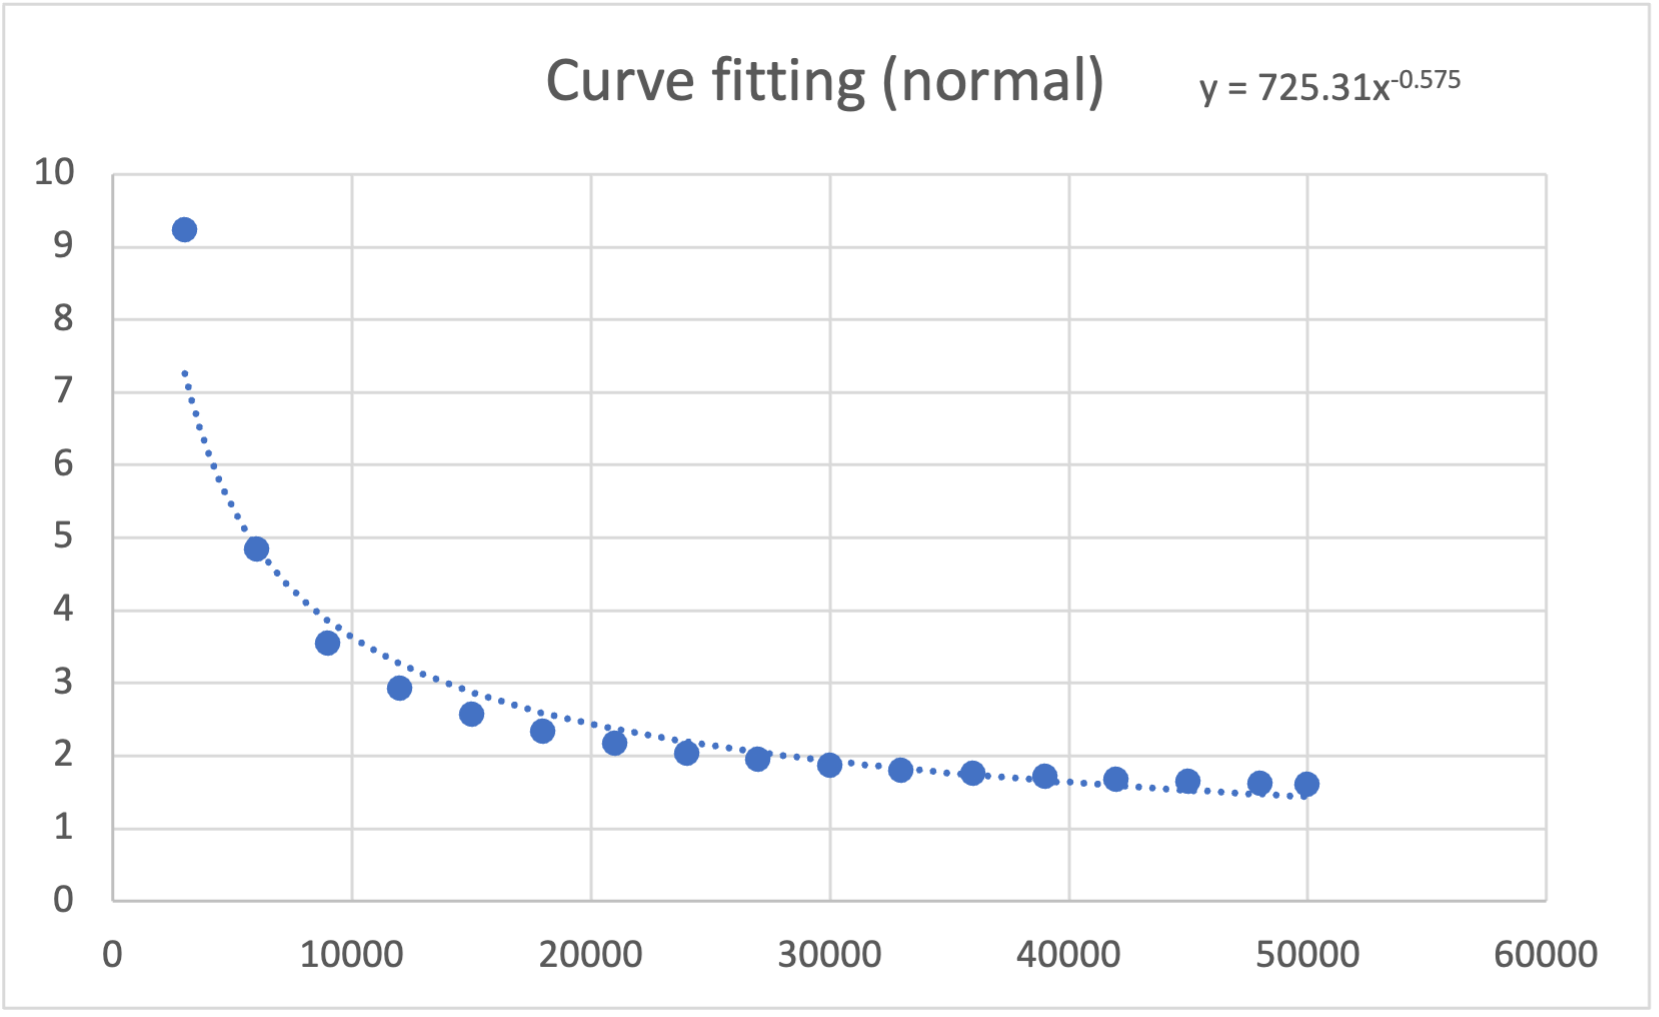
\includegraphics[width=0.8\textwidth]{chapters/images/curve_fitting_normal.png}
    \caption{Curve fitting (normal Data Center parameters)}
    \label{fig:curve_fitting_normal}
\end{figure}


On the other hand, in the second case, after setting the \emph{air distribution} parameter to \emph{perimeter cooling}, the same procedure was followed as described earlier, resulting in the following formula: \(y=1337.4x^{-0.623}\) and the corresponding chart is illustrated in figure \ref{fig:curve_fitting_modified}.
\begin{figure}[h]
    \centering
    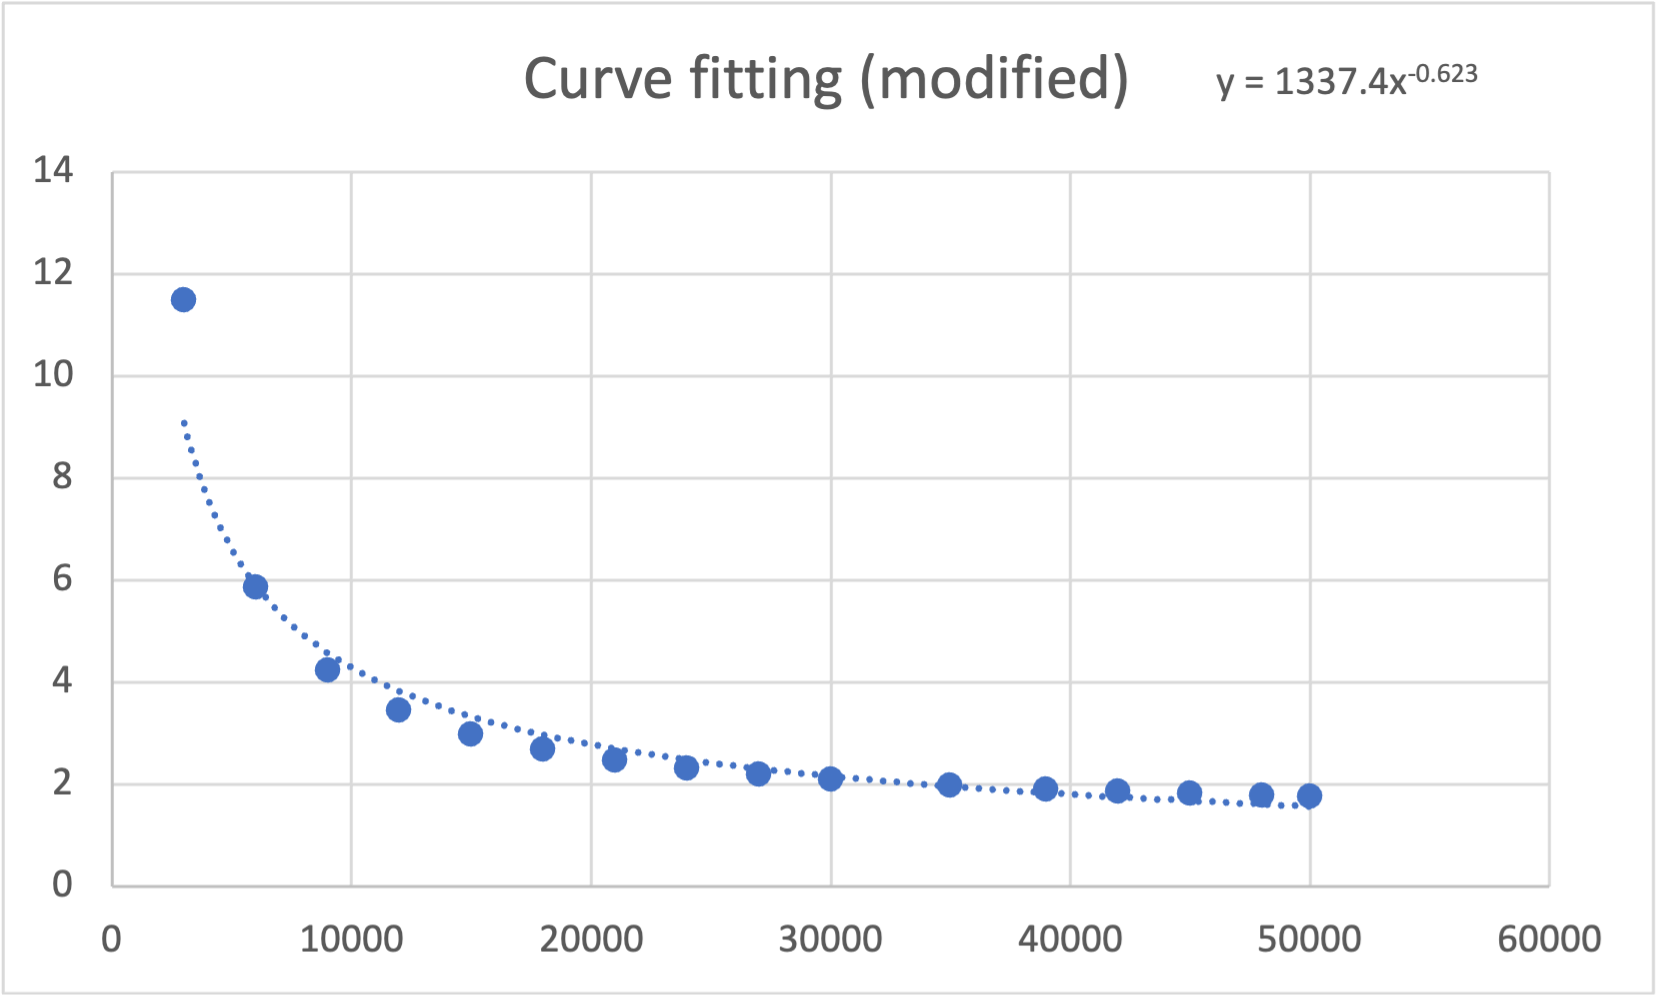
\includegraphics[width=0.8\textwidth]{chapters/images/curve_fitting_modified.png}
    \caption{Curve fitting (modified Data Center parameters)}
    \label{fig:curve_fitting_modified}
\end{figure}

\section{Executed simulations}
In order to examine the variation of PUE across several scenarios, multiple simulations under various conditions have been carried out. The simulations results, organized as described in Section \ref{subsection:simulationoutput}, are accessible in the \href{https://github.com/vincenzo-emanuele/masters-degree-thesis/tree/main/simulation_reports}{simulations\_reports} directory of the research work's repository. This directory comprises individual subdirectories corresponding to each conducted simulation. The following subsections provide descriptions of the individual conducted simulations. For each simulation a \emph{PUE} chart has been obtained using the formulas previously derived. 

\subsection{Normal load simulation} \label{subsection:normalload}
The first simulation has been performed keeping a constant load of about 40\% for the whole simulation time. This scenario is purely theoretical and does not account for load fluctuations, but it provides an insight into the \emph{PUE} values throughout the normal load periods. 
\begin{figure}[h]
    \centering
    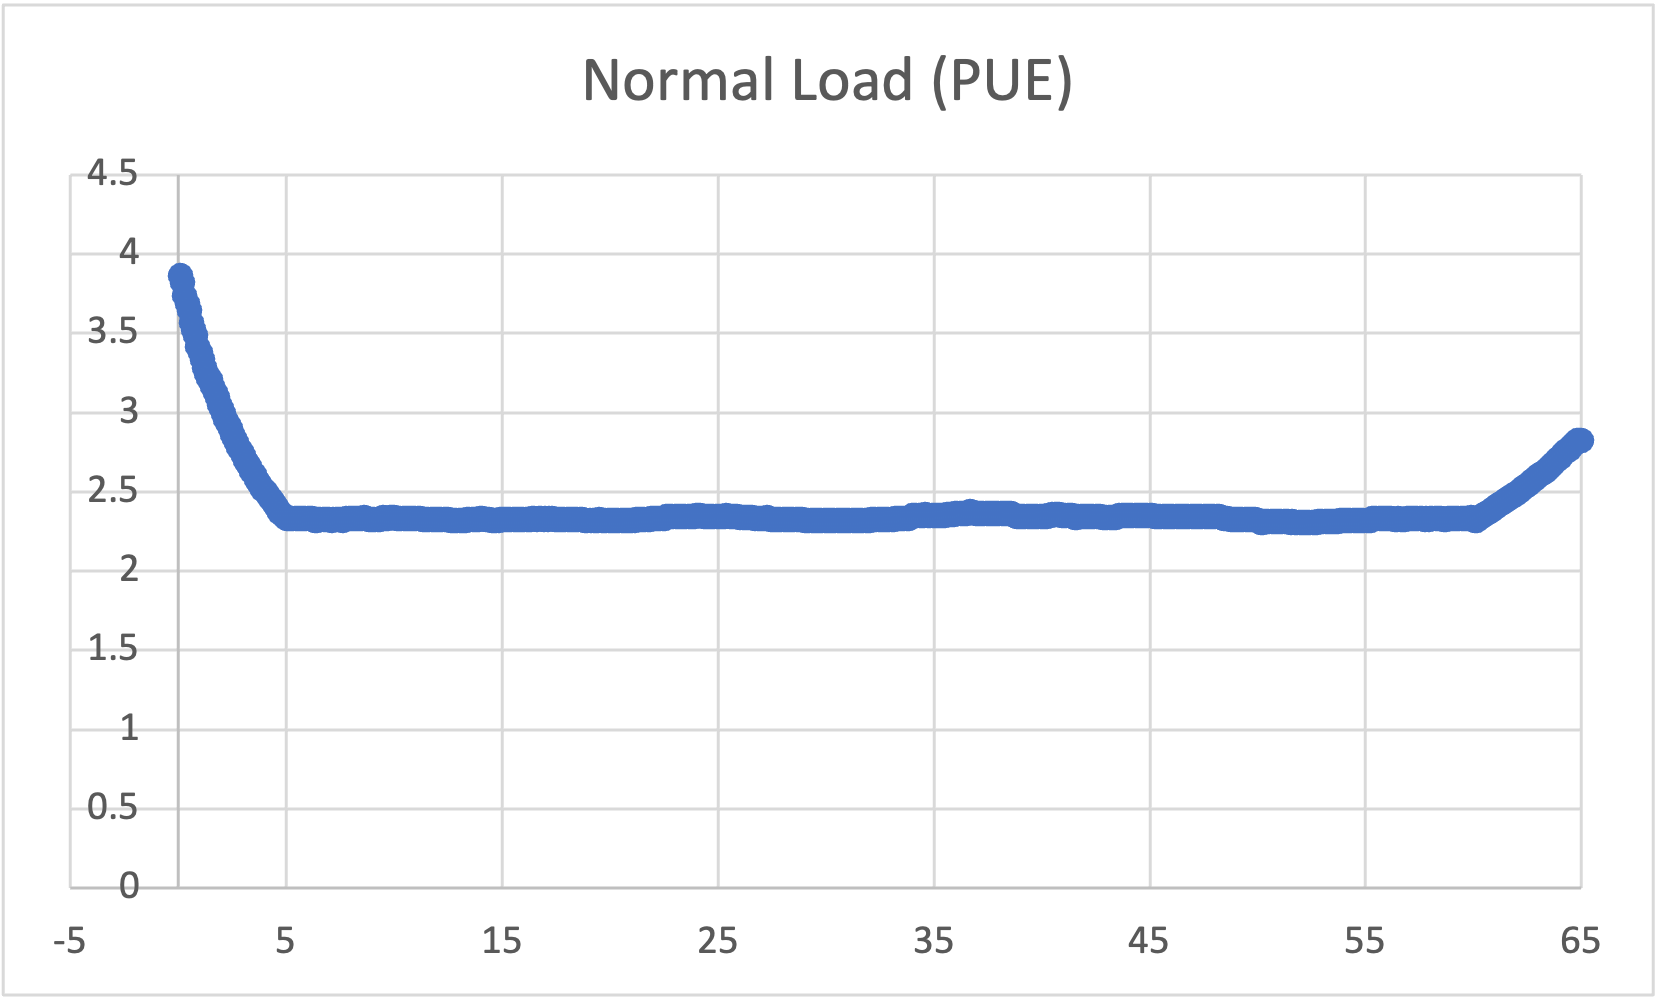
\includegraphics[width=0.6\textwidth]{chapters/images/normal_load_pue.png}
    \caption{Normal Load (PUE)}
    \label{fig:normal_load_pue}
\end{figure}
Figure \ref{fig:normal_load_pue} shows \emph{PUE} variation throughout the simulation. It is apparent that after a first period of about 5 seconds, during which the Data Center becomes fully operational, it remains constant for the whole simulation time and its value is around \textbf{2.32}. 

\subsection{Fast DoS scenario simulation}
This simulation has been performed by modeling a scenario in which the load rapidly increases from a normal condition of 40\% to reach 100\%. Specifically, the load variation was managed as follows: at the beginning of the simulation, a single user was instantiated, requiring computational power around 40\% of the total capacity. At time 20.0, an additional user was added, increasing the computational power demand to 80\%. At time 30.0, a third user was added, utilizing the full computational power. Subsequently, at time 40.0, the last user was added. Figure \ref{fig:fast_dos_pue} shows \emph{PUE} variation throughout the simulation. It is apparent that as long as the Data Center load has not reached 100\%, the variation in \emph{PUE} is noticeable as there is a \textbf{23\% decrease} when the second user joins the Data Center (from 2.33 to 1.80) and a \textbf{6.66\% decrease} when the third user joins the Data Center (from 1.80 to 1.68); however, after reaching the peak, this variation disappears entirely. 
\begin{figure}[h]
    \centering
    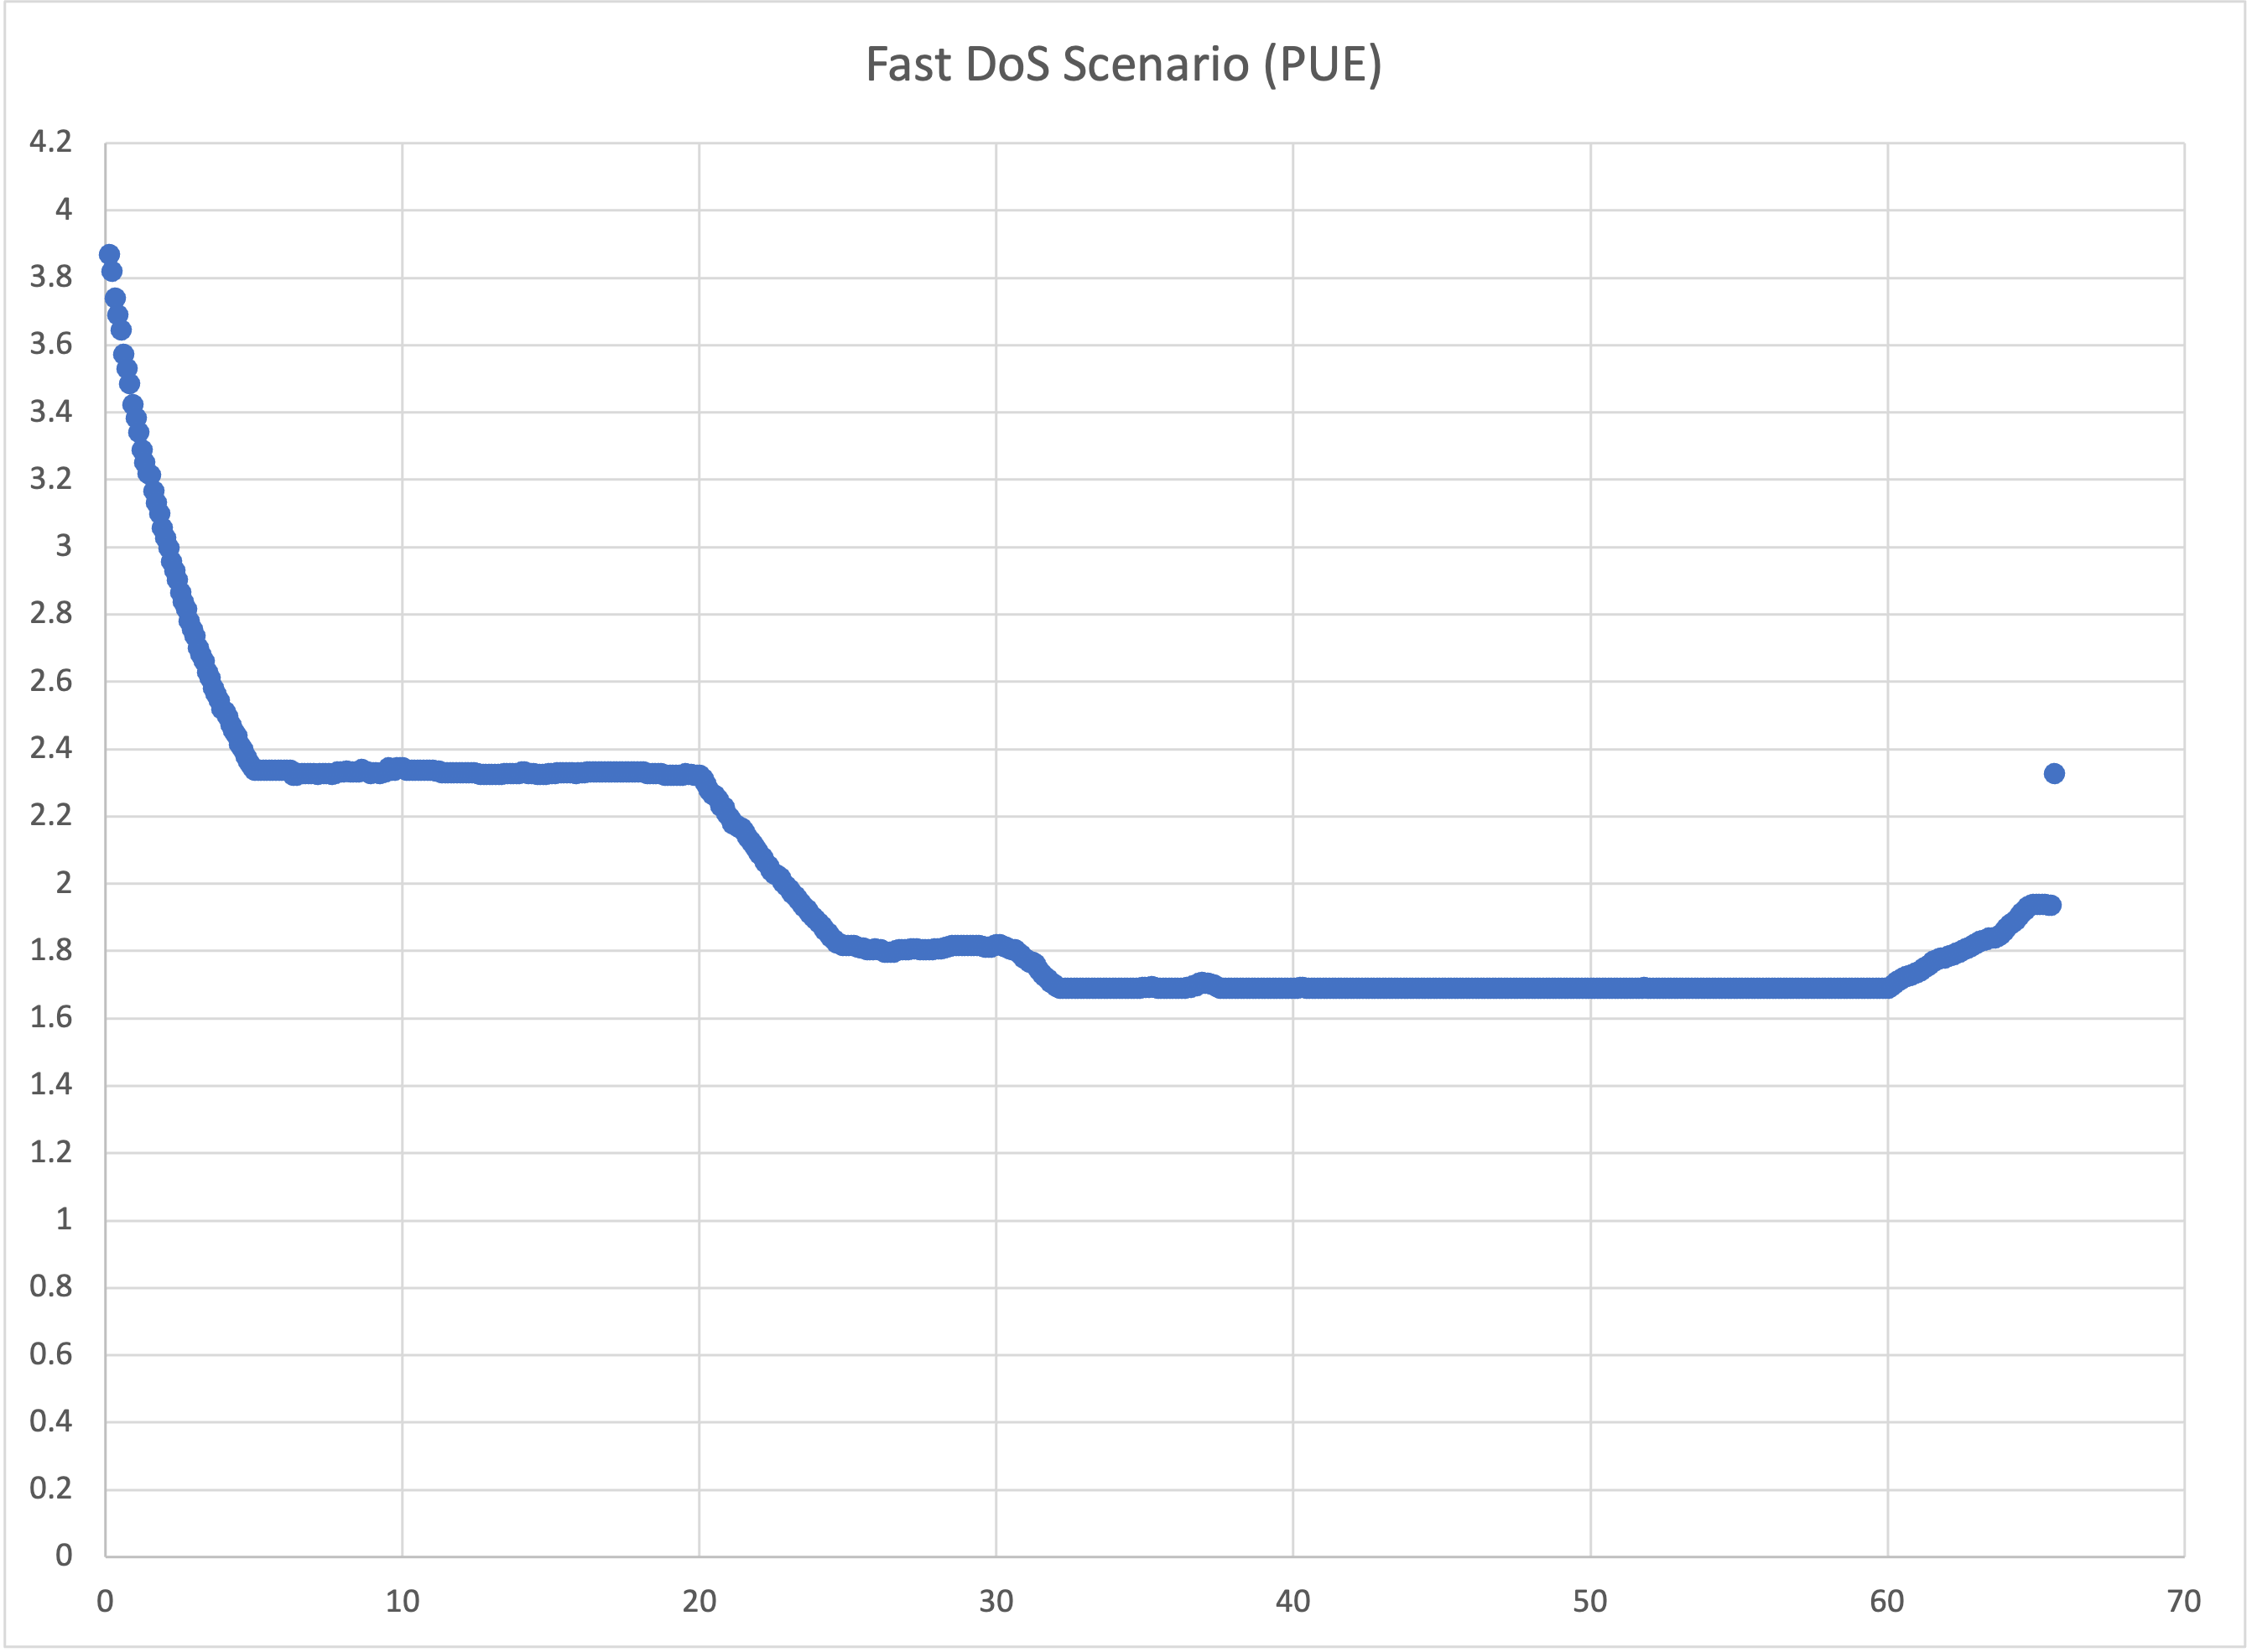
\includegraphics[width=0.6\textwidth]{chapters/images/fast_dos_pue.png}
    \caption{Fast Denial of Service Scenario (PUE)}
    \label{fig:fast_dos_pue}
\end{figure}

\subsection{Slow DoS scenario simulation}
This simulation has been performed by modeling a scenario in which the load slowly increases from a condition of 10\% to reach 100\%. Specifically, the load variation was managed as follows: at the beginning of the simulation, a single user was instantiated, requiring computational power around 10\% of the total capacity and then every 60 seconds a new user was instantiated for a total of 11 users throughout the simulation that lasted for 660 seconds. Figure \ref{fig:slow_dos_pue} shows \emph{PUE} variation throughout the simulation. It is evident that each load variation is definitely less observable compared to the fast \emph{DoS} scenario and is more pronounced as long as the Data Center load has not reached 60\% (around the time 360.0). \emph{PUE} variation ranges between 12\% and 4\%. 

\begin{figure}[h]
    \centering
    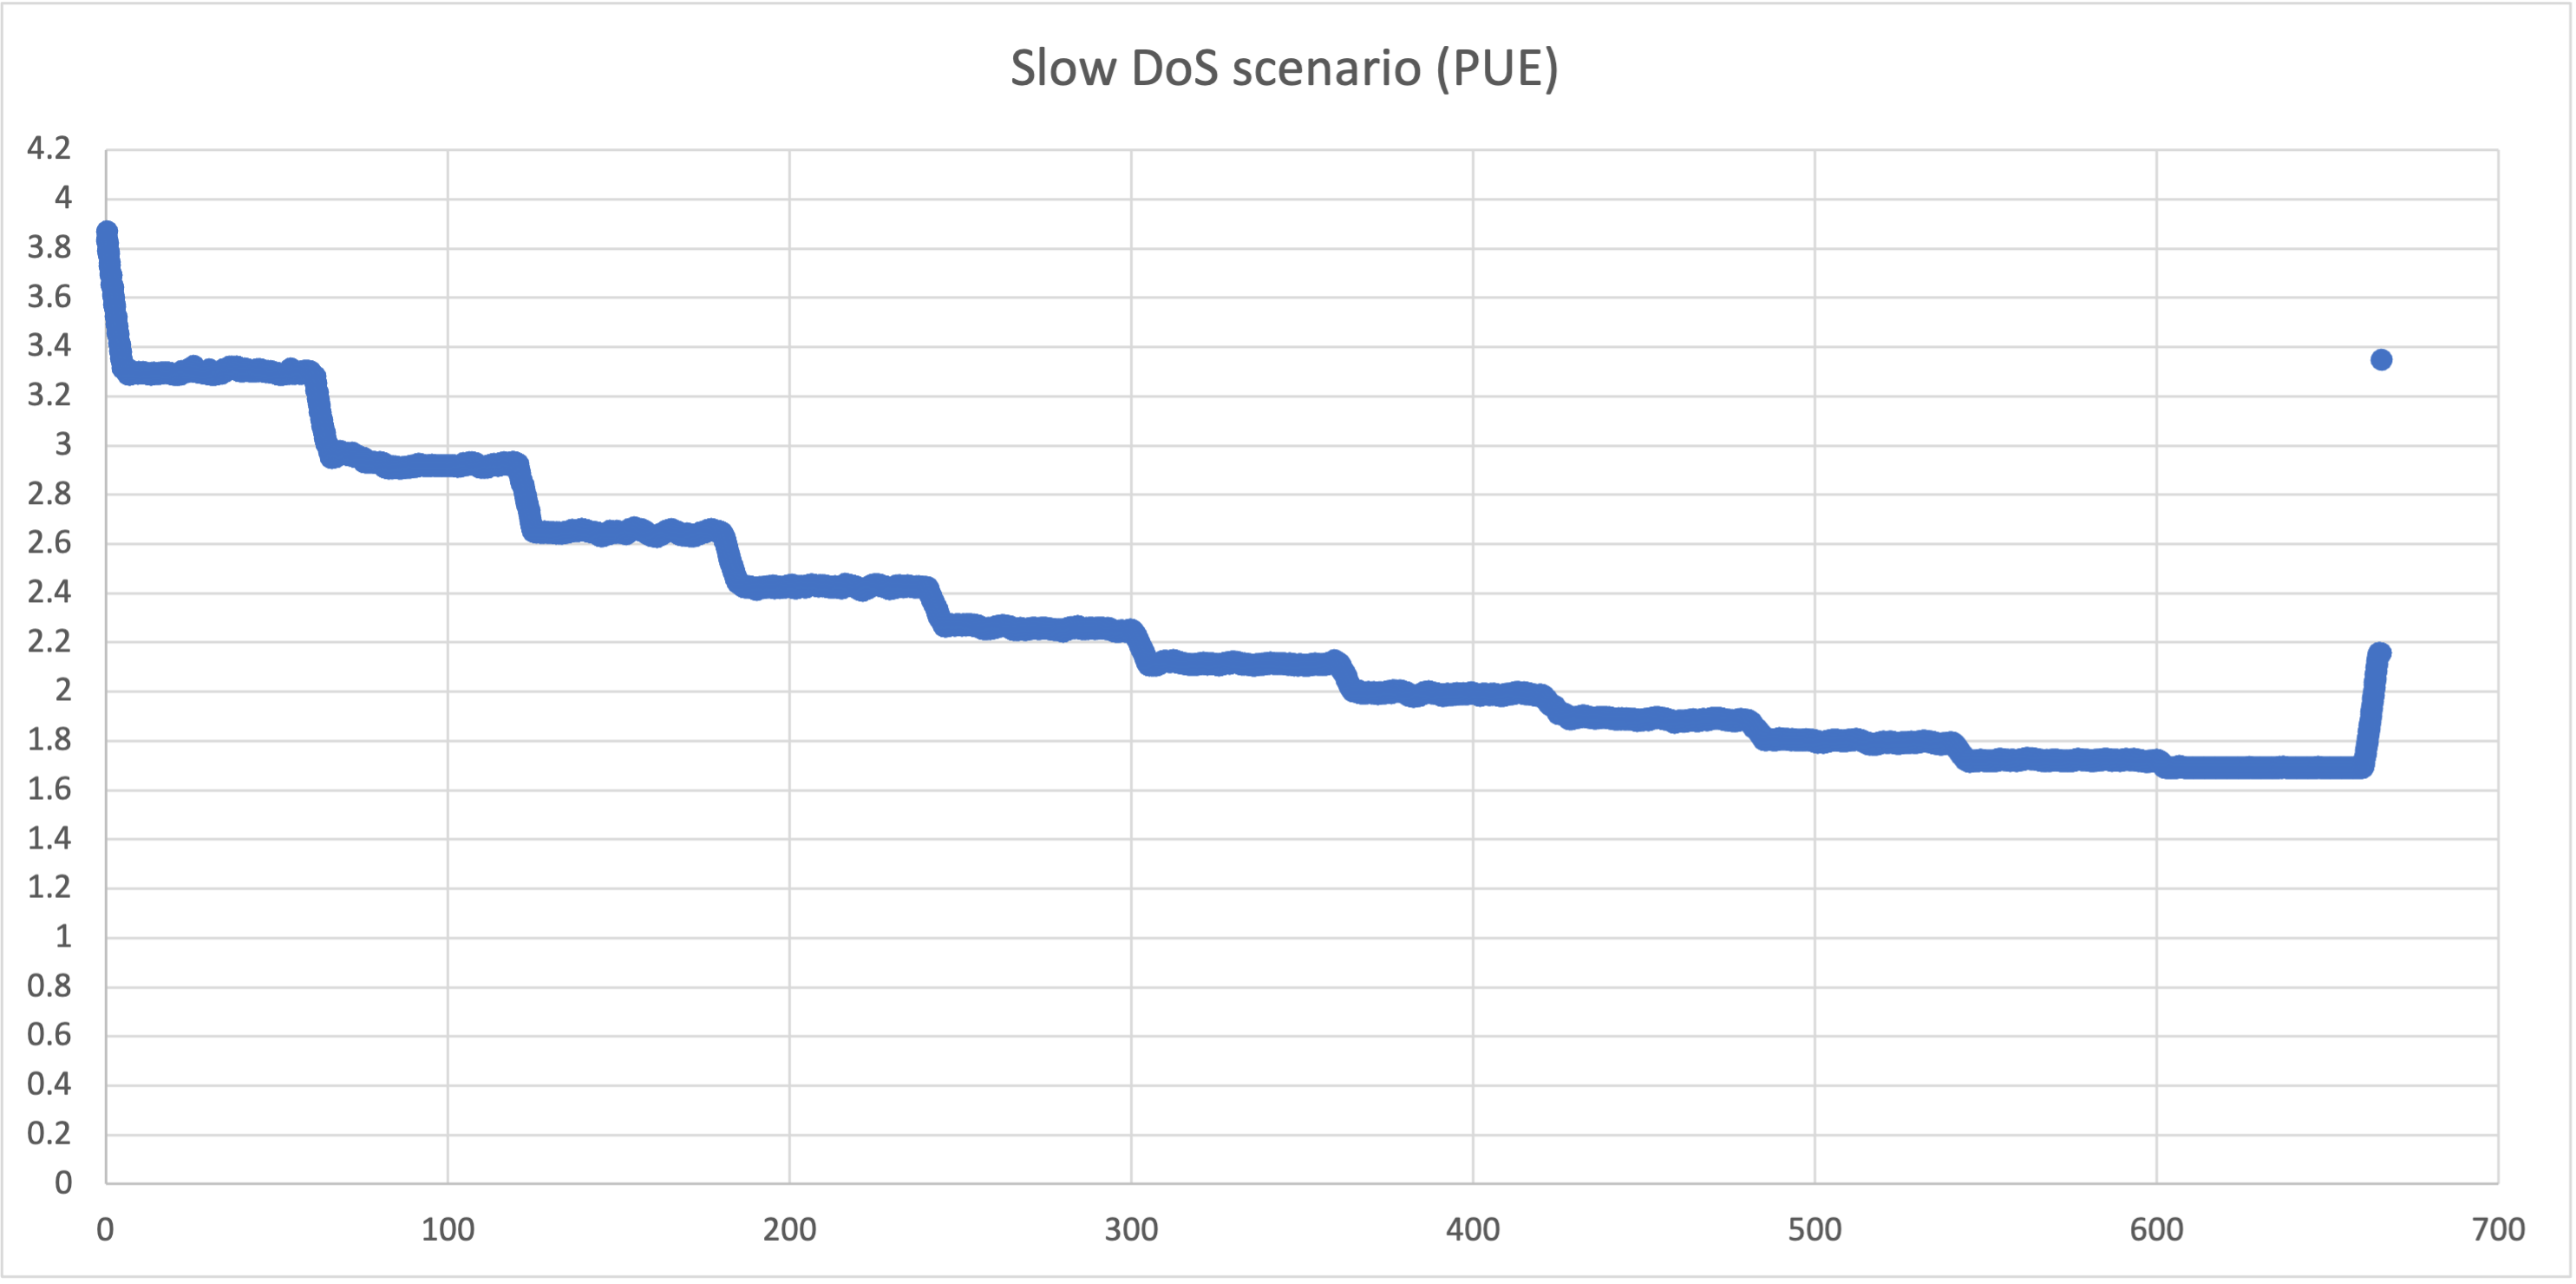
\includegraphics[width=0.6\textwidth]{chapters/images/slow_dos_pue.png}
    \caption{Slow Denial of Service Scenario (PUE)}
    \label{fig:slow_dos_pue}
\end{figure}

\subsection{Cooling system attack scenario simulation} \label{subsection:coolingsystemattack}
In order to simulate the scenario where the cooling system is attacked as outlined in subsection \ref{subsection:coolingsystemattack}, data from the previously conducted simulations were utilized. Specifically, the data from the silent \emph{DoS} scenario were used as it covers all the workload conditions. The \emph{PUE} was calculated using both the formula applicable under normal conditions and the formula applicable under the cooling system attack scenario. The variation in \emph{PUE} was then observed. Figure \ref{fig:pue_comp} illustrates the comparison of \emph{PUE} trends throughout the whole simulation, showing the difference between the Data Center when it has not experienced a cooling system attack and when it has. \emph{PUE} value variation ranges \textbf{between 17.4\% and 10.5\%}.
\begin{figure}[h]
    \centering
    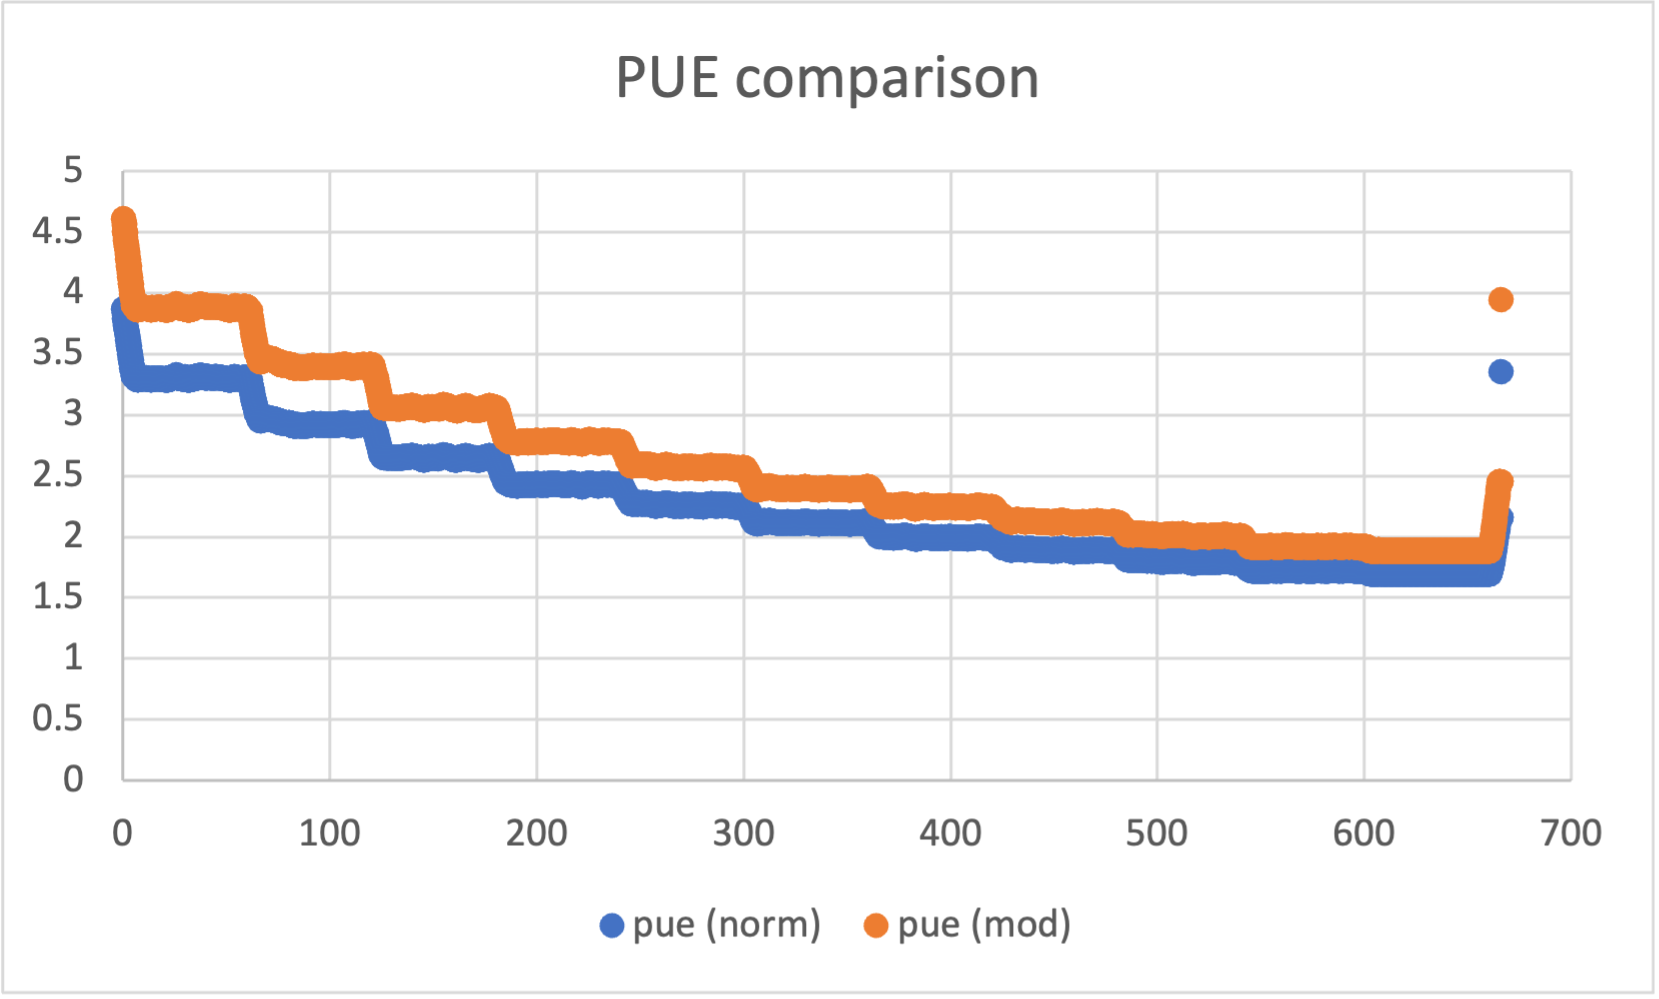
\includegraphics[width=0.6\textwidth]{chapters/images/pue_comp.png}
    \caption{PUE comparison}
    \label{fig:pue_comp}
\end{figure}



\section{Results}
Once the simulations are done and the graphs showing changes in \emph{PUE} are obtained, it is important to look at the data to figure out if the \emph{PUE} parameter is really helpful to detect the studied attacks. The following subsections aim to provide both reflections about the collected data placing them in real-world contexts and a comparison with the current state of the art will be carried out to contextualize the proposed approach within existing detection techniques.

\subsection{PUE utilization in DoS scenarios}
The simulation conducted to model the fast \emph{DoS} scenario, reveals a noticeable percentage change in \emph{PUE}, which is observable up to a certain point, and then gradually diminishes until it disappears completely. The reason behind this phenomenon can be attributed to the shape of the \emph{PUE} curve illustrated in figure \ref{fig:pue_curve} (gathered from the \href{https://www.se.com/ww/en/work/solutions/system/s1/data-center-and-network-systems/trade-off-tools/data-center-efficiency-and-pue-calculator/}{\emph{Schneider Electric SE} tool}). After reaching 55\% of the maximum supported capacity by the Data Center, it becomes less steep compared to the portion ranging from 0\% to 55\%. It then further flattens after reaching 75\%, stabilizing at approximately 1.70. This explains the sudden variation in \emph{PUE} during the time the Data Center takes to become operational. The collected data suggests that the time it takes for the Data Center to start accommodating a sudden drastic load change (from 40\% to 80\% of total capacity) is around 5 seconds. During this period, there is an increase in the overall energy consumption of about 11000 W (23\% \emph{PUE} decreasement). However, the scenario is quite different when transitioning from 80\% to full resource saturation. In that case, the change is about 5000 W in 5 seconds (6.66\% \emph{PUE decreasement}), and it eventually disappears with further computational resource demands. 
Furthermore, in the case of a slow DoS situation, the PUE variation becomes less noticeable. In the analyzed scenario, the maximum observable percentage variation is 12\% when the load goes from 10\% to 20\%. However, as the load increases, the variation becomes lower due to the reasons discussed earlier. Therefore, the PUE can definitely be used as a parameter for detecting rapid and noisy DoS attacks, up to the point of reaching the peak supported load. There is no need to use static values or thresholds; it is enough to observe a significant \emph{PUE} variation within a certain time interval. In the studied case, this interval is 5 seconds, as mentioned before, which is the time the Data Center takes to accommodate load changes (independent of simulation time), while the significance of the \emph{PUE} variation needs to be established based on the context. A non-trivial problem lies in distinguishing between a \emph{DoS} attack and an increase in load due to legitimate traffic that results in a significant \emph{PUE} variation. The distinction between these two scenarios cannot be solely accomplished through monitoring the \emph{PUE}, but requires additional methodologies, such as a profile of energy consumption during different times of the day and year. Based on these profiles, the percentage variation threshold is dynamically adjusted. To understand the approach based on variable thresholds, it is possible to consider the following practical scenario. Let's consider a data center that supports real-time communication activities (including meetings) of a company operational from 9 to 18. Let's suppose that after performing a profiling activity, it becomes evident that the majority of traffic is concentrated between 9:30 and 12:30, and between 15:00 and 17:30. Therefore, it is reasonable to expect a sharp decrease in PUE around 9:30 and 15:00. Hence, a variation recorded around those times is presumably not indicative of a DoS attack. Let's assume that generally, during active hours, around 45\% of the available computational resources are utilized on average. In this case, it is reasonable to consider that a potential PUE variation around or exceeding 20\% could be a symptom of a DoS attack. Finally, suppose that during the night and holidays, the utilization of computing resources hovers around 5\%. In that scenario, even a 10\% PUE variation could signify a DoS attack, as it would mean reaching 13\% of the computing resources' utilization in the data center, namely more than double the observed load. It is important to take into account that the numbers mentioned are purely indicative and come from results obtained through simulations conducted on a simplified model of a data center. To implement such a system in a real-world scenario, it is necessary to consider data obtained from that specific real system.

\begin{figure}[h]
    \centering
    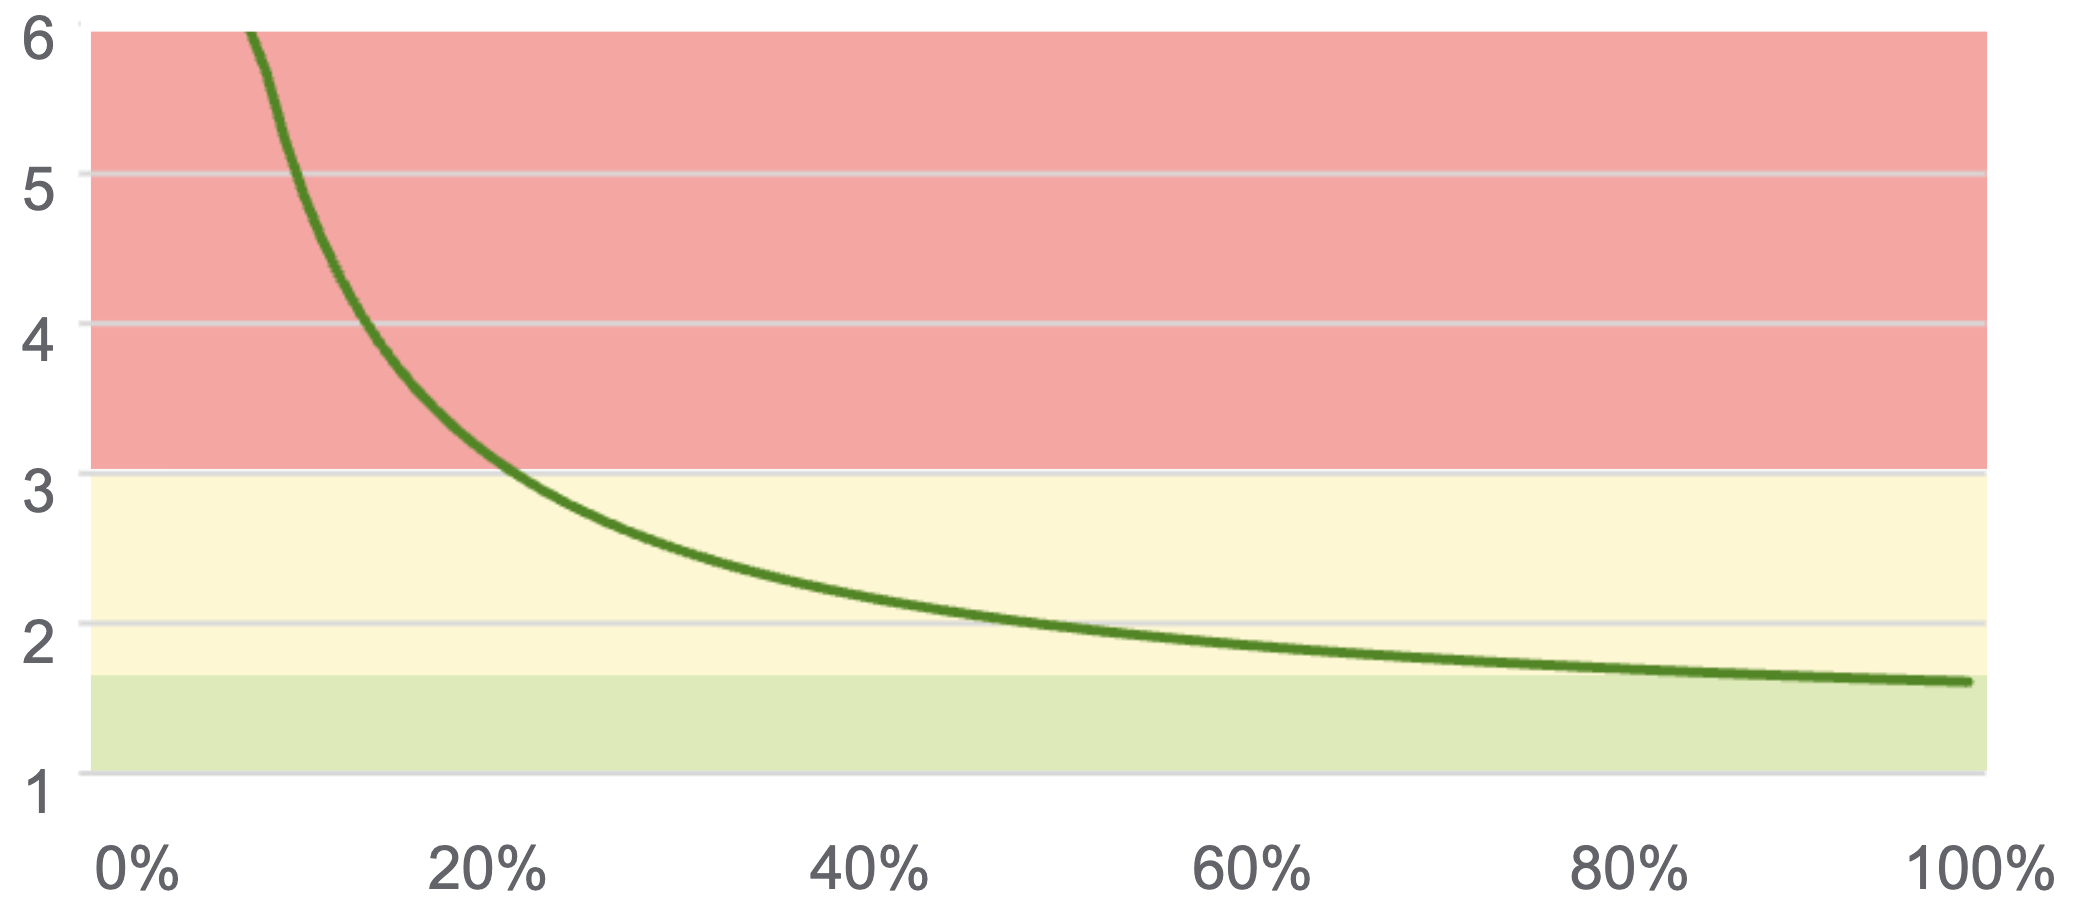
\includegraphics[width=0.8\textwidth]{chapters/images/pue_curve.png}
    \caption{PUE curve}
    \label{fig:pue_curve}
\end{figure}

\subsection{PUE utilization in cooling system attack scenarios}
As highlighted by the results obtained and described in subsection \ref{subsection:coolingsystemattack}, unlike the case of the \emph{DoS} scenario, the difference in \emph{PUE} variation is well observable regardless of the load conditions. Once again, the reason behind this phenomenon can be attributed to the nature of the curve describing the \emph{PUE}, which, in the case of an attack on the close-coupled cooling system, is shifted. Figure \ref{fig:pue_curves_comp} illustrates the curve obtained through curve fitting for the scenario where no attack is occurring and the curve obtained through curve fitting for the scenario with an attack on the cooling system, presented on the same graph.
\begin{figure}[h]
    \centering
    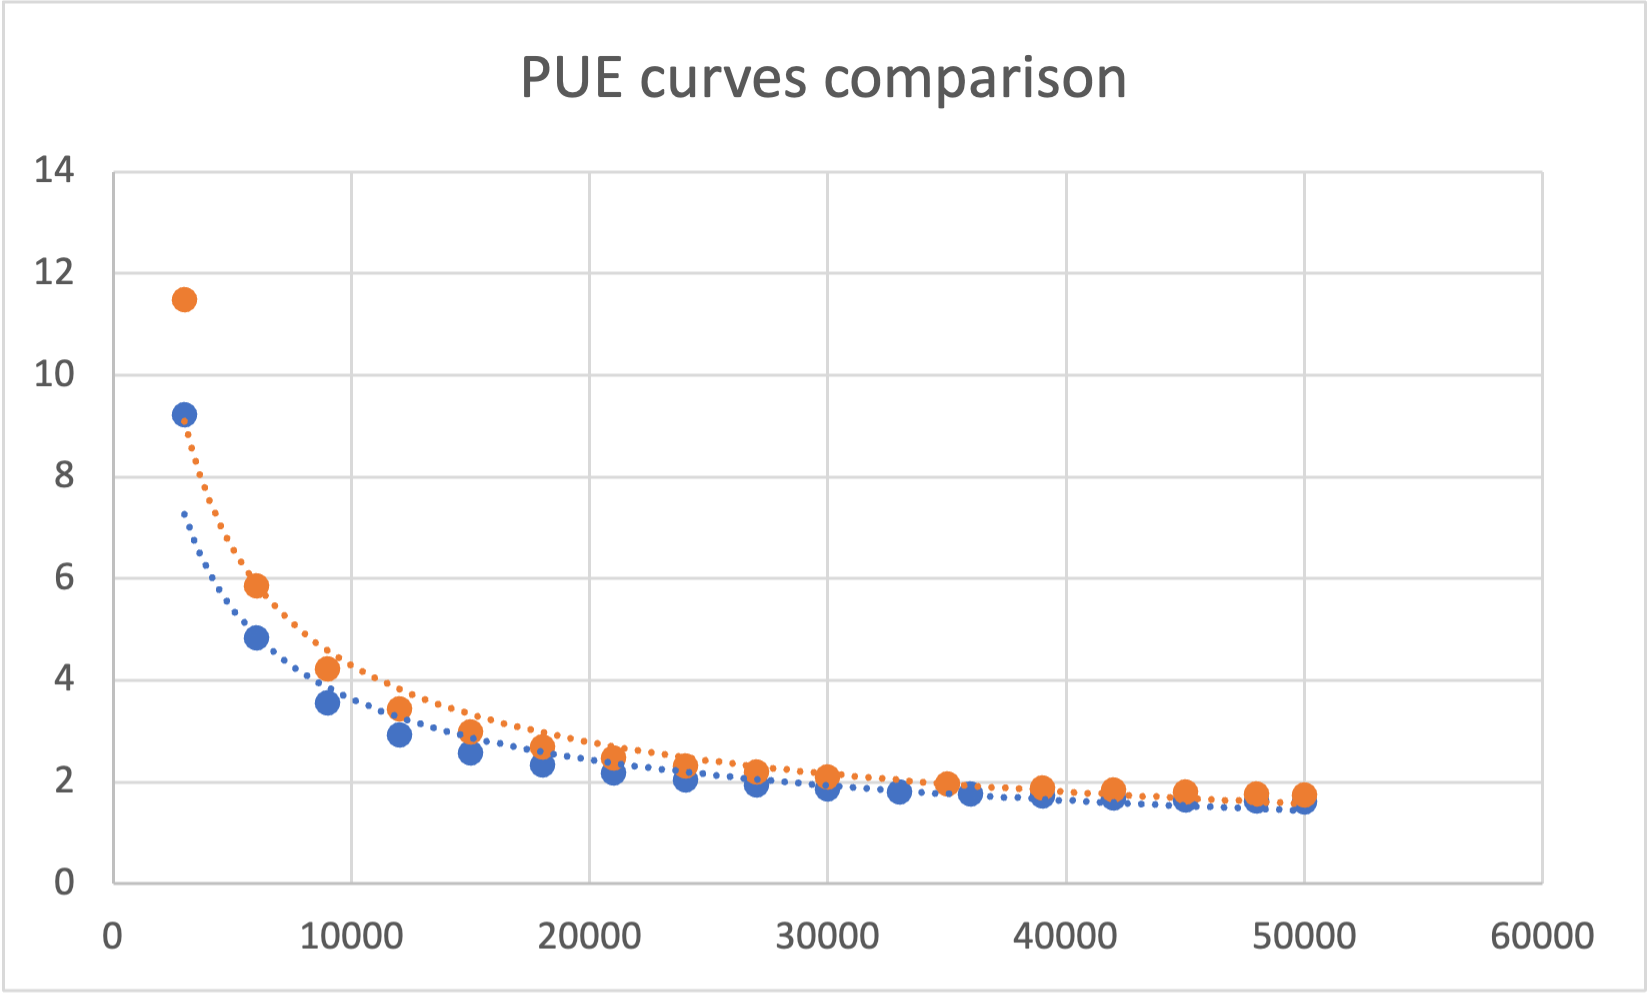
\includegraphics[width=0.8\textwidth]{chapters/images/pue_curves_comp.png}
    \caption{PUE curves comparison}
    \label{fig:pue_curves_comp}
\end{figure}
Although the two curves seem to overlap at some point, the study has shown that even under maximum load conditions a difference in \emph{PUE} of 10\% is observable. Unlike the \emph{DoS} case, where detecting the attack involves monitoring a shift on the same curve that tends to flatten out, in this scenario, the problem is reduced to determining which curve the points observed during runtime belong to. If they belong to the curve that describes the scenario of an attack at the cooling system, it is reasonable to assume that an attack is occurring.
Referring to the real-world scenario described earlier, an attack that disables the close-coupled cooling system can be detected at any time of the day, even during peak operational hours of the Data Center. Unlike the previous case, in this scenario, it's not just the \emph{PUE} variation itself that needs to be observed but a variation while keeping energy consumption constant. Therefore, if the \emph{PUE} is expected to have a certain value around a specific level of energy consumption, a significant change in it (which depends on load conditions) under the same energy consumption conditions can be indicative of an attack. Highlighting once again, the numbers mentioned are approximate and derived from simulations on a simplified Data Center model. To deploy this system in a real-world scenario, specific data from the actual Data Center must be considered. The scatter graph shown in figure \ref{fig:pue_variation_cooling} displays the percentage change in PUE between the two scenarios, starting from a 10\% load and reaching the maximum load. It is noticeable that this variation ranges between 10\% and 18\%, making the \emph{PUE} a valid parameter for attack detection.

\begin{figure}[h]
    \centering
    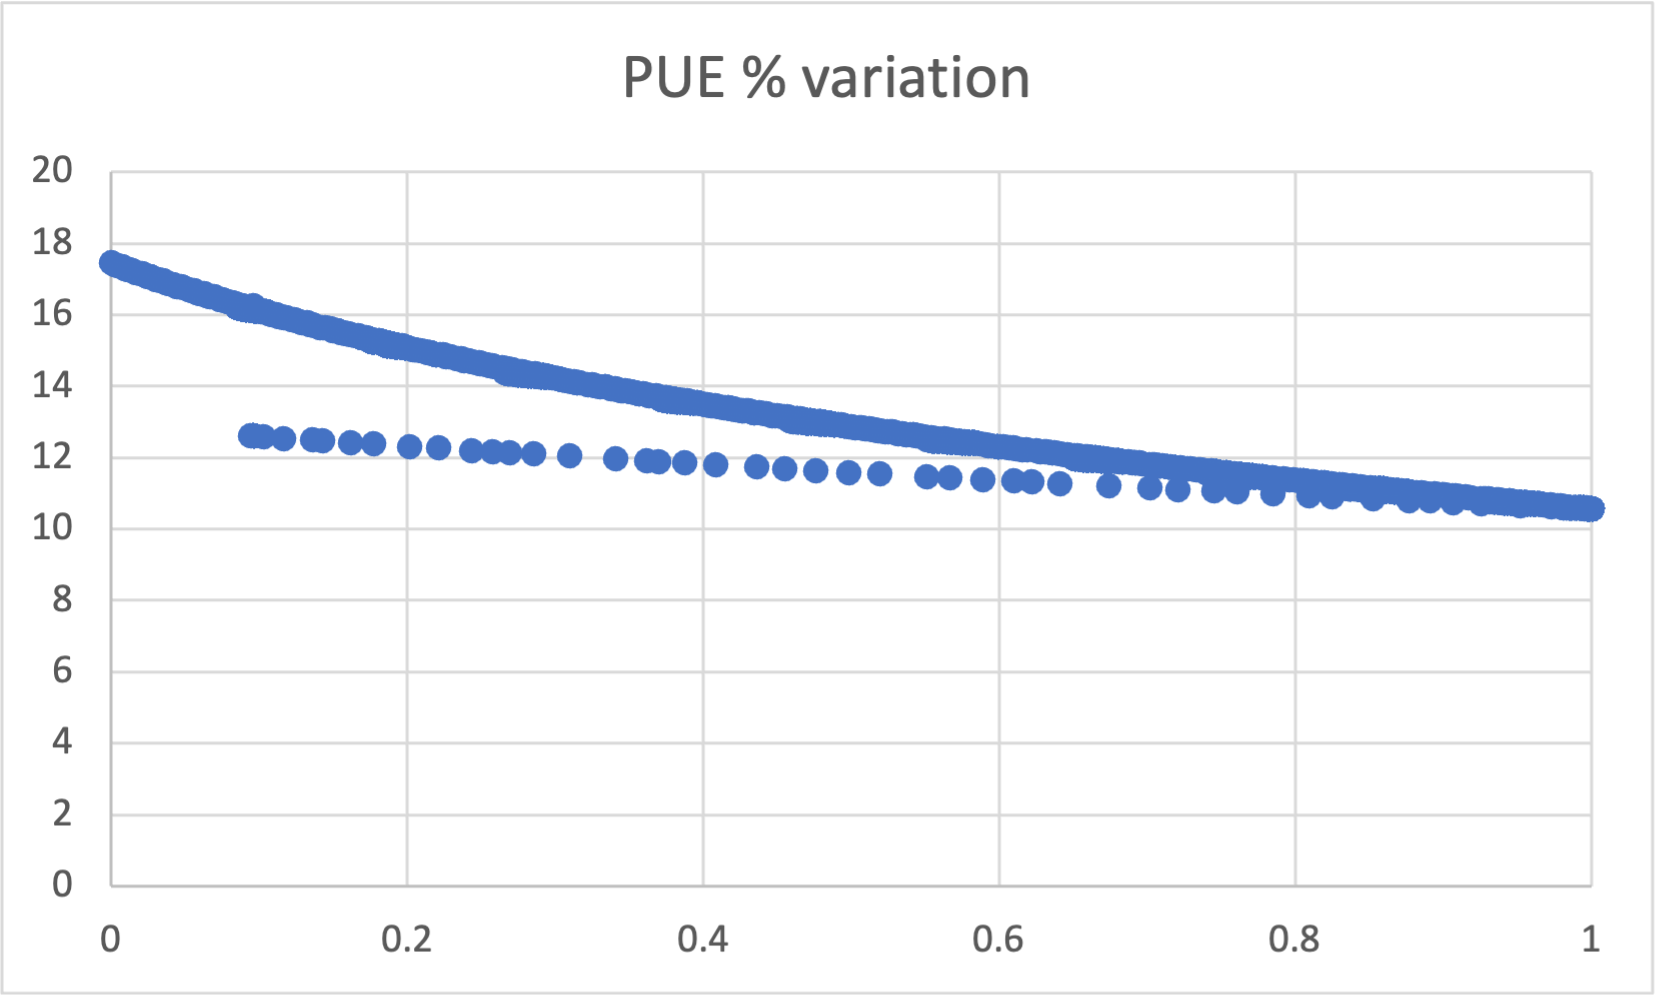
\includegraphics[width=0.8\textwidth]{chapters/images/pue_variation_cooling.png}
    \caption{PUE percentage variation}
    \label{fig:pue_variation_cooling}
\end{figure}

\subsection{Comparison with the State of the Art}
After explaining the limits within which \emph{PUE} results effective to detect the described attacks, it is useful to contextualize these approaches within the current state of the art solutions. These approaches do not need specific equipment for \emph{PUE} calculation; a wattmeter and one of the \emph{PUE} calculation techniques explained in Subsection \ref{subsection:puecalculation} are enough. In comparison to conventional anomaly detection methods outlined in Section \ref{section:ids}, this detection technique stands out because it operates without the need to understand or inspect network traffic. For this reason, it does not require artificial intelligence techniques or models training in order to work. However, as explained before, this approach has inherent limitations, especially during peak load moments when distinguishing between an attack and a normal load increase can become difficult. Therefore, as highlighted before, it is crucial to complement this technique with a comprehensive consumption profile. In general, the proposed technique can be used in synergy with existing state of the art solutions, functioning as an early warning system for potential \emph{DoS} attacks. In cases where the detection threshold is not sufficiently high, a traffic inspection technique should be used.






